\chapter{Impact du vieillissement dans les pays de l'union européenne}
\paragraph{}Si tout le monde est d’accord sur les constats tiré au premier chapitre, il n’en va pas de même pour les impacts que ce vieillissement pourrait avoir sur la société. Le premier impact qui vient à l’esprit est bien entendu le problème de financement des retraites. Une autre problématique fort proche de la première est l’augmentation probable des dépenses de santé. Lorsque presque 35\% de la population aura plus de 65 ans et que la population active passera de 60\% à 50\% c’est à dire une diminution de 17\% de celle-ci, nous sommes en mesure de nous demandé si il y aura encore assez de travailleur pour faire tourner l’économie.  

\section{L'avenir du financement des retraites}
\paragraph{}Pour comprendre le problème que vont poser les pensions, ils faut d’abord parler du système de retraite par répartition qui est majoritaire en Europe~\citep{system_retraite}. Ce système se base sur les cotisations de la population active pour financer le pension des retraités, en d’autre terme la somme des cotisations est répartie entre tout les pensionnés~\citep{retraite_repartition}. Sachant cela, il devient vite évident que le vieillissement de la population va poser un problème. Inexorablement, la proportion de population active part rapport aux pensionnés va diminuer. Il sera impossible de garantir le montant des pensions sans augmenter la somme cotisée.  

\paragraph{}Dans le chapitre précédent, nous avons vu que le degré de dépendance va passer de 23\% à 33\% en 2060, ce qui est en soit déjà inquiétant. Mais si on regarde de plus prêt cette mesure n’est pas très réaliste. A l’heure actuelle l’âge moyen de début d’activité n’est pas à 15 ans mais tourne plutôt autour de 20~\citep[pp.27]{eul} et l’âge moyen de départ à la retraite est plutôt entre 61 et 62 ans en 2009~\citep{eurocompar}. Le graphe \ref{real_dep} montre le taux de dépendance pour une population active allant de 20 à 61 ans et de 20 à 64 ans. Il est intéressant de tenir compte des chiffres du chômage pour avoir une meilleur idée de la population réellement active. Le taux actuel est de 9,8\% en moyenne dans l’Europe des 28~\citep{chaumage}. Il ne prétend pas montrer des chiffres exactement mais des tendances plus proches de la réalité. 



\begin{figure}[h!]
    \begin{center}
        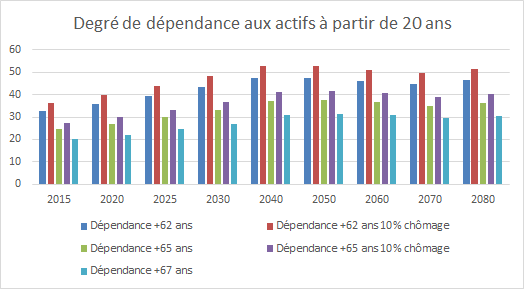
\includegraphics[scale=0.9]{document/real_dep.png}
        \caption{Calcul du niveau de dépendance des personnes agées sur base de la population active à partir de 20 ans basé sur les projections EUROPOP2013. source: Eurostat~\citep{eurostat_europop13}}
        \label{real_dep}
    \end{center}
\end{figure}

\paragraph{}Les chiffres sont plutôt alarmants, si on est à prêt de 33\% a l’heure actuelle, c’est-à-dire que trois personnes cotise pour une. On dépasse le 50\% en 2040, c’est à dire que seulement deux personnes devront cotisé pour une, le maintien des pensions devrait passer une augmentation de 50\% des cotisations. Bien entendu, si on table sur le plein emploi et un âge de le retraite effectifs à 67 ans, le degré de dépendance plafonne à 31\% en 2040. L’augmentation de l’âge de la retraite semble inévitable comme le concède Héran~\citep[pp.18]{heran}.

\paragraph{}Hervé Le Bras~\citep[pp.19-39]{heran} prétend que cela ne sera pas nécessaire. En prenant, la population active de 20 à 61 ans moins 10\% de chômage on arrive à 260 millions d’actif dans l’Europe de 28 en 2015. On serait encore loin du compte car elle en compterait un peu moins de 215 millions~\citep[pp.36]{heran}. Pour l’auteur, il “suffirait” d'activer les membres inactifs de la société comme les personnes âgée de plus de 55 ans et les femmes au même niveau que les hommes de moins de 55 ans pour maintenir l’équilibre. Les avis sur la solution diverge, mais il y a un consensus pour s’accorder sur le fait que le système de retraite européen sera en faillite si rien ne change. 

\section{Impact sur les dépenses de santé}
\paragraph{}L’impact du vieillissement sur les dépenses de santé son plus compliquée à évaluer. D’après Herve Le Bras~\citep[pp.31]{heran} les dépenses de santé on augmenté de 4,2\% par an au cours des 25 dernière années. Néanmoins, cela ne serait en grand partie pas dû au vieillissement de la population.  Il part de l’hypothèse que les personnes âgées de plus de 60 ans dépensent trois fois plus que les autres. Une hypothèse comme nous le verrons à relativiser. En 2015, il y a 23\% de personnes de plus de 60 ans, il y en aura 35\% en 2050.


\paragraph{}En prenant le coût moyen pour une personne de moins de 60 à 1 et donc le coût d’une personne de plus de 60 à 3, il arrive à un coût moyen de 1,468 en 2015 ($23,4 * 3 + 76,6 * 1$) et 1,7 en 2050 ($35 * 3 + 65 *1$). Ce qui correspond à une augmentation de 0,3\% par an, on est donc bien loin des 4,2\%. Et cette augmentation sera probablement encore plus faible car une augmentation de l’espérance de vie va aussi de paire avec une augmentation du niveau de vie en bonne santé et donc d’une augmentation des dépenses de santé plus tardive. 

\paragraph{}Le rapport “aeging report”~\citep{ageing} décrit deux effets qui pourrait mettre en péril la viabilité du système de santé des pays européen. Le premier est l’augmentation de la longévité sans l’augmentation de la longévité en bonne santé qui ferait donc augmenter les dépenses. La seconde, qui rejoint la logique du système de retraite, est l’augmentation de la proportion de personne âgée par rapport à la proportion de personne cotisante~\citep[pp.116]{ageing}.   

\paragraph{}Mais tout de suite, les auteurs reconnaissent que l’augmentation de la durée de vie active et l’augmentation de la durée de vie en bonne santé pour atténuer les deux effets. En effet, si l’augmentation de la durée de vie en bonne santé augmenter de la même manière que la durée de vie, l’augmentation des dépenses par habitant dans le domaine de la santé pourrait être nulle.  Ils expliquent, comme dans l’article Le Bras que le vieillissement de la population n’aurait pas contribué à augmenter les dépenses de santé dans les proportions communément admises.~\citep[pp.116]{ageing} 

\paragraph{}Le report fait de nombreuses projections basée sur différentes hypothèses de longévité et de longévité en bonne santé.  Le rapport projette dans une scénario moyen, une augmentation de 1,1\% de la part de PIB dans les dépenses de santé. Mais, dans un scénario ou seul le facteur démographique les dépenses n’augmenteraient que de 0,2\%~\citep[pp.18]{ageing}. 

\paragraph{}En conclusion, si les dépenses vont augmenter, le vieillissement de la population n’en sera qu’une cause minime. L’évolution technologie et les progrès de la médecine en revanche y joue un grand rôle~\citep[pp.120]{ageing}. 

\section{Diminution de la population active}
\paragraph{}Dans le chapitre précédent, nous avons vu que d’après les projections EUROPOP13, la population de l’Europe des 28 va croître jusqu’en 2050 mais ce n’est pas le cas de la population potentiellement active (de 20 à 64 ans). Celle-ci va décroître chaque année comme le montre le graphe \ref{active} de 306 millions en 2015 à 265 millions en 2080. L’augmentation de l’âge de la pension de 2 ans ne changera pas vraiment le donne, la population active passerait alors de 318 millions à 277 millions. 

\begin{figure}[h!]
    \begin{center}
        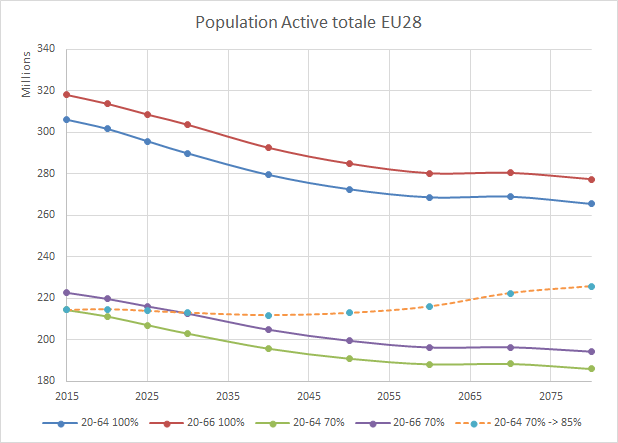
\includegraphics[scale=0.7]{document/active.png}
        \caption{Projection de la population active de 2015 à 2080 dans l'Europe des 28. source: Eurostat~\citep{eurostat_europop13}}
        \label{active}
    \end{center}
\end{figure}

Dans ces circonstances, si le PIB par habitant moyen n’augmente pas le PIB des pays européen pourrait diminuer de 14\% avec toutes conséquence néfaste d’une déflation comme par exemple une augmentation de la dette publique relative au PIB.\footnote{Pour un moment total de dette inchangé une diminution du PIB implique automatiquement une augmentation de la dette par rapport au PIB.} Cependant, il est possible d’atténuer les effet démographique comme le propose Le Bras, en activant une partie de la population non active~\citep[pp.36]{heran}. la ligne pointillée orange sur le graphe \ref{active} montre les effets d’une augmentation linéaire de l’activité de 70\% à l’heure actuelle~\citep{eurostat_emploi} vers 85\% en 2080. Contrairement à l’augmentation de l’âge de la retraite, l’activation des non actif permettrait de garder une proportion de travailleur constant voir en légère augmentation après 2050. 

\section{Autres impacts}
\paragraph{}En dehors de la problématique des retraites et des soins de santé, ils existent de nombreux autres impacts. 

\paragraph{}Nous avons beaucoup parler des retraités, mais la population active vieillit également, actuellement l’âge moyen de la population active est de 42 ans\footnote{ En prenant l’age moyen des personnes de 20 à 64 ans.~\citep{eurostat_europop13}}, il montera jusqu’à 43 ans en 2025. Ce vieillissement additionné à la diminution du nombre d’actif pourrait entraîner une inadéquation entre les compétences disponible et celles nécessaires~\citep[pp.10]{thesis} car les plus jeunes sont souvent les mieux formés aux nouvelles technologies. Ceci représentera un défit pour les entreprises. 

\paragraph{}Les personnes âgées ont aussi des comportement assez différent d’une population plus jeune. Si la présence d’un vote vieux n’est pas avéré~\citep[pp.10]{heran}, il est clair que les personnes âgées consomment différemment, ils consomment plus de service de voyage, d’hôtel, restaurant, bien entendu dans tout le secteur de la santé,  en service de maisons de retraites mais aussi dans les assurances, les banques. On peut parler d’économie grise~\citep[pp.11]{thesis}. 

\paragraph{}Dans une catégorie plus sociale, l’allongement de la durée de vie ainsi que la baisse du taux de fécondité change totalement le visage des familles. On passe d’un modèle pyramidale (grand-parents < parents < enfants) à une pyramide inversée  (grand-parents > parents > enfants) ainsi que la présence de nouvelle génération les arrière-grand-parents et bientôt les arrière arrière grand parents~\citep[pp.13]{thesis}.

\paragraph{}Il y a encore de nombreux impacts sociaux et économique que nous n’avons pas abordé ici. Il est clair que le vieillissement a des impacts non négligeable sur notre société. Dans le chapitre suivant, nous allons analyser certaines pistes pour permettre de contrebalancer les effets ou montrer comment la société peut et devra s’adapter à cette nouvelle situation. 
 

 
